\documentclass[conference]{IEEEtran}
\IEEEoverridecommandlockouts
\usepackage{cite}
\usepackage{amsmath,amssymb,amsfonts}
\usepackage{graphicx}
\usepackage{textcomp}
\usepackage{xcolor}

\title{
\vspace{1cm}
{
\includegraphics[width=0.15\textwidth]{1.jpg} \\ 
7447 BCD - Seven segment Display Decoder Assignment} }

\author{Patnam keerthi\\ Roll No: FWC22306 \\ patnamkeerthi4545@gmail.com}

\begin{document}
\maketitle

\section{ABSTRACT}
This paper shows how to use the 7447 BCD-Seven segment Display Decoder to learn Boolean logic using Arduino Uno.

\section{COMPONENTS}
The required components list is given in Table: I, and the seven-segment display is shown in Fig. 2. The IC 7447 diagram is shown in Fig. 1.
\vspace{0.3cm}

\begin{table}[htbp]
\centering
\begin{tabular}{| c | c | c |}
\hline
Components & Value & Quantity \\
\hline
IC & 7447 & 1 \\
\hline
Seven segment display & & 1 \\
\hline
Arduino & UNO & 1 \\
\hline
Jumper Wires & & 10 \\
\hline
Breadboard & & 1 \\
\hline
\end{tabular}
\vspace{0.3cm}
\caption{\label{tab:widgets} Components List}
\end{table}

\begin{figure}[htbp]                           
\centering                            
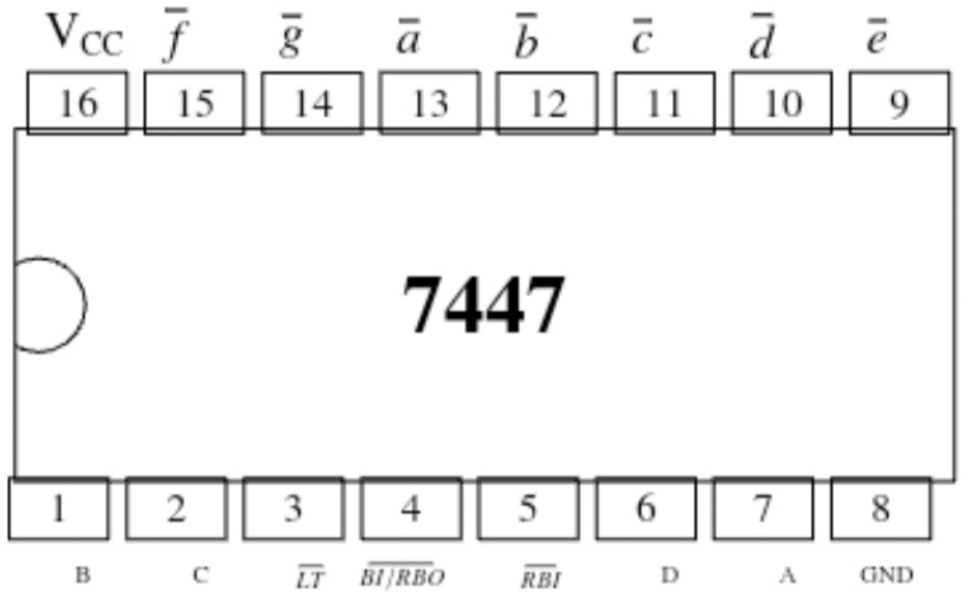
\includegraphics[width=0.5\textwidth]{2.jpg}             
\caption{\label{fig-1:Gates} IC 7447}           
\end{figure}

\begin{figure}[htbp]                           
\centering                                 
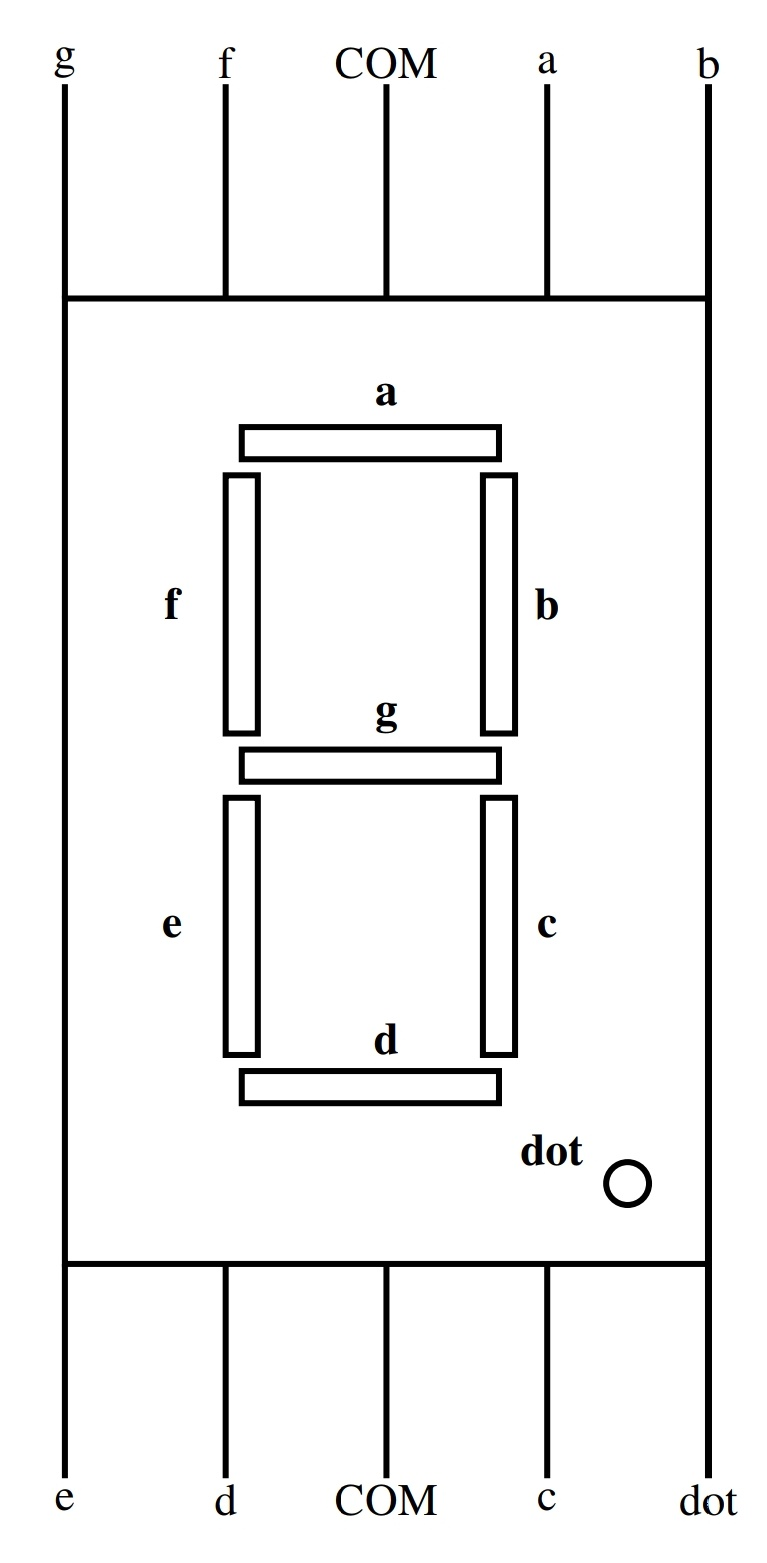
\includegraphics[width=0.3\textwidth]{3.jpg}                                           
\caption{\label{fig-2:Gates} Seven Segment Display}               
\end{figure}

\section{PROCEDURE}
\begin{enumerate}
\item Make the connections of 7447 IC and the seven-segment display as shown in Fig. 3.
\item Make the connections of 7447 IC and Arduino Uno as shown in Fig. 4.

\begin{figure}[htbp] 
\centering 
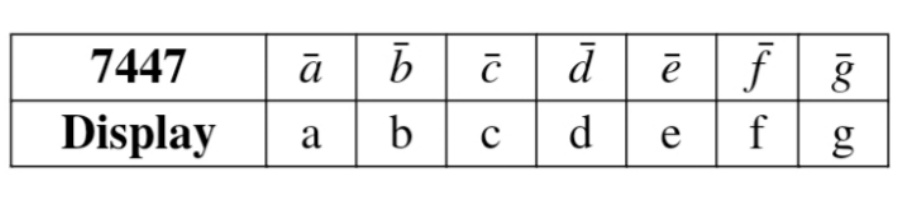
\includegraphics[width=0.3\textwidth]{4.jpg}
\caption{\label{fig-3:Gates} Circuit Setup 1}    
\end{figure}

\begin{figure}[htbp]                     
\centering                           
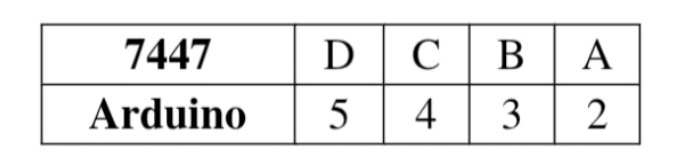
\includegraphics[width=0.3\textwidth]{5.jpg}                                 
\caption{\label{fig-4:Gates} Circuit Setup 2}         
\end{figure}

\item Truth table for incrementing from $0$ to $9$ in the seven-segment display is shown in Table II.

\begin{table}[htbp]
\centering
\begin{tabular}{| c | c | c | c | c | c | c | c |} 
\hline
$Z$ & $Y$ & $X$ & $W$ & $D$ & $C$ & $B$ & $A$ \\
\hline
0   & 0   & 0   & 0   & 0  & 0 & 0  & 1 \\
0   & 0   & 0   & 1   & 0  & 0 & 1  & 0 \\
... & ... & ... & ... & ... & ... & ... & ... \\ 
\hline
\end{tabular}
\vspace{0.15cm}
\caption{\label{tab:widgets} Truth Table for Seven-Segment Display}
\end{table}

\item Execute the Arduino code without any errors.
\item Upload the code into the hardware setup using Arduino IDE.
\end{enumerate}

\section{RESULTS}
\begin{enumerate}
\item Download the code from the link below and execute it to see the output as shown in Fig. 5.
\item https://github.com/Pranaykuma/FWC-1/blob/main/7447/main.cpp
\end{enumerate}

\begin{figure}[htbp] 
\centering 
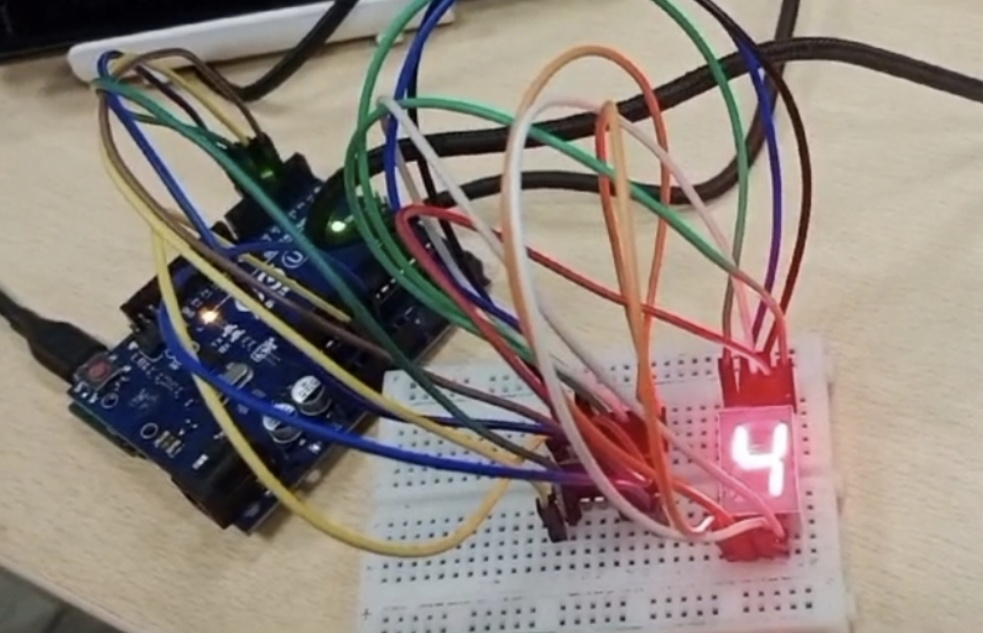
\includegraphics[width=0.4\textwidth]{6.jpg}
\caption{\label{fig:Gates} Output Example}    
\end{figure}

\section{CONCLUSION}
Hence, the implementation of the 7447 IC and Seven-segment display using Arduino UNO is complete.
\end{document}
